\section{Subspace Clustering}
The main idea of subspace clustering is to identify subspaces of a high dimensional space to allow better clustering than the original (full) space. This is opposed to e.g. PCA, which projects the original space onto a new subspace, which may can be hard to interpret for the user.

Two different subspace clustering approaches will be discussed. First, the grid-based approach will be discussed, after which the density-based approach will be discussed. Note that, only bottom-up approaches will be considered in this paper.

We will adopt the following notation: Let $\mathcal{A} = \{A_1, \dots, A_d\}$ be a set of domains, and $\mathcal{S} = A_1 \times A_2 \times \dots A_d$ a $d$-dimensional numerical space containing $n$ points $p_1, \dots, p_n$. Let $A_1, \dots, A_d$ be the dimensions (attributes) of $\mathcal{S}$.

\subsection{Grid-based approach}
The key idea of grid-based subspace clustering is to partition the $\mathcal{S}$ into axis-parallel grid structure starting in 1-dimensional space. The grids forms hyper-rectangular \textit{units} (cells) for which we find the number of points in each. Only the units that exceeds a certain threshold are retained, called \textit{dense units}. Next, adjacent dense units will be merged to form so called \textit{candidate dense units} (CDUs), which will be used to find clusters in higher dimensional subspaces. The goal is then to describe the clusters using a minimal description in the form of DNF (\textit{Disjunctive Normal Form}) expressions.

\subsubsection{CLIQUE}
CLIQUE is a bottom-up grid-based subspace clustering algorithm that uses the monotonicity property as the clustering criterion, which is similar to the well-known Apriori algorithm.
\begin{lemma}\label{lem:mono}
    If a collection of points $S$ is a cluster in a $k$-dimensional subspace, then $S$ is also a part of a cluster in any $(k-1)$-dimensional projections of this space.
\end{lemma}
Proof can be found in \cite{clique}.

First, $\mathcal{S}$ is partitioned into equal-sized $\varepsilon$ (input parameter) intervals, creating axis-parallel rectangular units. Hereafter, the dense units are found in the 1-dimensional space. The dense units are then merged to form CDUs in the 2-dimensional space, thus reducing the search space using Lemma \ref{lem:mono}. That is, CDUs in any $k$ dimensions are obtained by merging the dense cells in $(k-1)$ dimensions which share the \textit{first} $(k-2)$ dimensions. The procedure to merge dense cells continues unitil no more CDUs are generated. However, if a dense unit exists in $k$ dimensions then all of its projections in a subset of the $k$ dimensions that is $O(2^k)$ different combinations, are also dense. Therefore the running time of the algorithm is exponential in the highest dimensionality of any dense unit. However, using a pruning technique suggested in \cite{clique}, where the authors suggest to prune subspaces with low coverage, that is the number of points that the dense units cover in a subspace. However, this comes with a cost as it may prune subspaces that may contain clusters.

A cluster is a maximal set of connected dense units in $k$-dimensions. Two $k$-dimensional units $u_1, u_2$ are \textit{connected} if they have a common face in the $k$-dimensional space, that is the two units share $k-1$ dimensions. or if they are connected by a common cell. That is, there exists another $k$-dimensional unit, say $u_3$, such that $u_1$ is connected to $u_3$ and $u_2$ is connected to $u_3$.

A region in $k$ dimensions is an axis-parallel rectangular $k$-dimensional set. We are only interested in those regions that can be expressed as unions; henceforth all referencs to a region mean such unions. A region can be expressed as a DNF expression on intervals of the domains $A_i$.

We aim to make a minimal description of a cluster which will be a non-overlapping covering of the cluster. An example is given in Figure \ref{fig:dense_cells_and_regions}, where the grid size given by $\varepsilon$ is 0.05, where the minimal description of the cluster is $A \cup B$ and has the DNF expression: $((0.05 \le A_1 < 0.15) ~\wedge~ (0.10 \le A_2 < 0.20)) ~\vee~ ((0.10 \le A_1 < 0.20) ~\wedge~ (0.05 \le A_2 < 0.15))$.
\begin{figure}[H]
    \vspace*{-0.5cm}
    \centering
    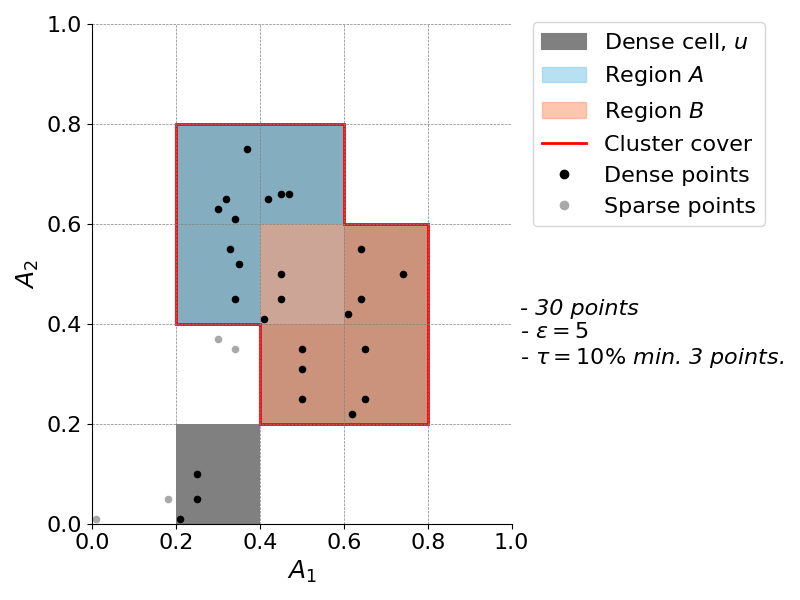
\includegraphics[width=0.3\textwidth]{figures/dense_cells_and_regions.png}
    \caption{Illustration of a dense unit $u$ and two overlapping dense regions $A$ and $B$.}
    \label{fig:dense_cells_and_regions}
    \vspace*{-0.5cm}
\end{figure}

\subsection{MAFIA}
MAFIA is an extension to CLIQUE where the grid sizes are adaptive meaning that the grid sizes are not fixed but are automatically determined by an algorithm. The idea is to cosim-2012ncentrate the portions of the data space, as having more points a more likely to be part of a cluster region enabling minimal length DNF expressions. The overall intention is not to rely on the input parameters CLIQUE uses do not use on the pruning technique as noted in cite{clique}, this could result in lost information. The algorithm is described in more detail in Section \ref{sec:mafia}.

\subsection{Density-based approach}
A big drawback of grid-based methods is that the rely on the grids. In Figure \ref{fig:dense_cells_and_regions} we see that the due to the ragid grid structure we might miss cluster points closely to the dense cells due to non-rectangular cluster shape. Furthermore, This is a limitation of grid-based methods. Density-based methods do not have this limitation, as they do not rely on grids. Instead, they rely on the density of the data points. A well-known density-based clustering algorithm is DBSCAN \cite{dbscan}.


Description of SUBCLU and describe how it relates to DBSCAN.